\chapter{Analysen}\label{ch:method}

\section {Voruntersuchungen}
\subsection{Ausgangssituation}
\subsection{Vorgehensweise}
\subsection{Ergebnisse}

\paragraph{Image List}
Jedes Listenelement muss einzeln hinzugefügt werden. Listen haben immer große Dimensionen, unglaublicher Zeitaufwand.

\begin{center}
  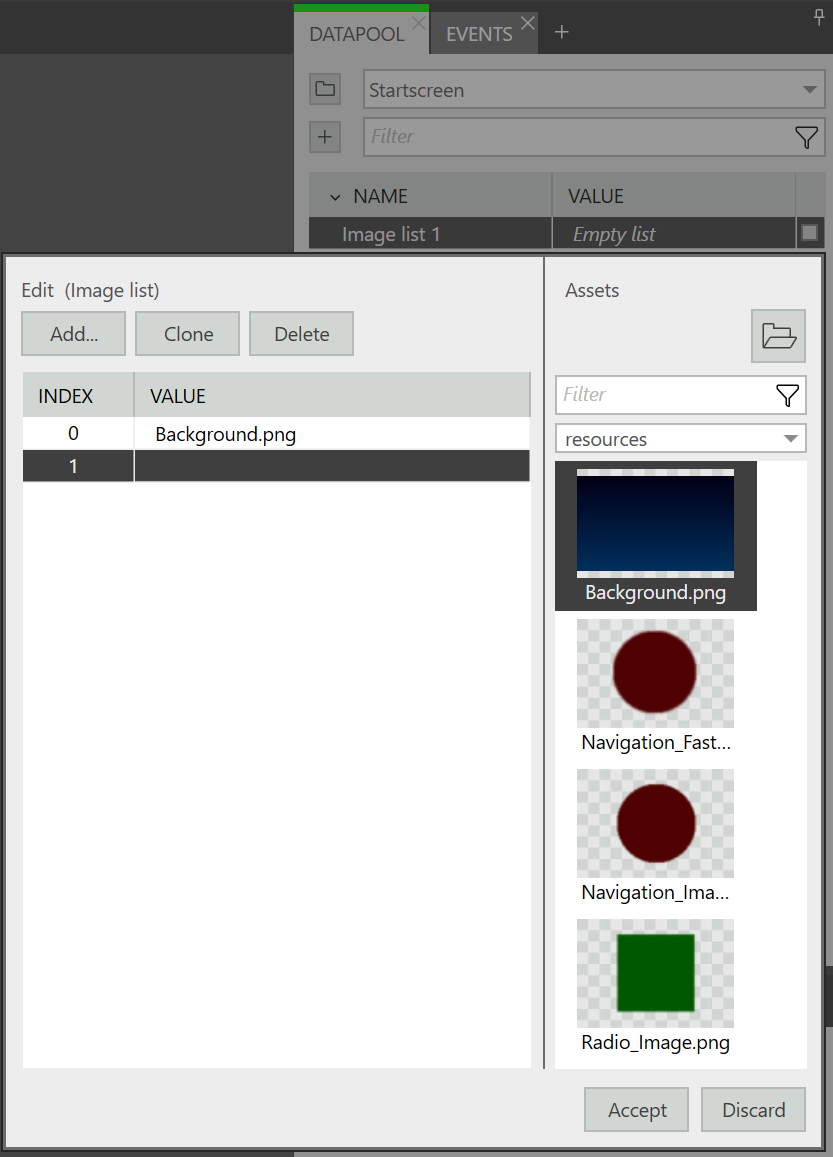
\includegraphics[scale=0.5]{figures/ImageList.png}
  \captionof{figure}{Usability - Schwäche Image List}
  \label{fig:ImageList}
\end{center}


\paragraph{Navigation}
Wird ein neues Element in der View hinzugefügt wird der Baum in der Naviagtion nicht automaisch ausgeklappt. Das Element muss zum umbenennen gesucht werden. Automatisches ausklappen und markieren des eingefügten Objektes zur Umbenennung.

\begin{center}
  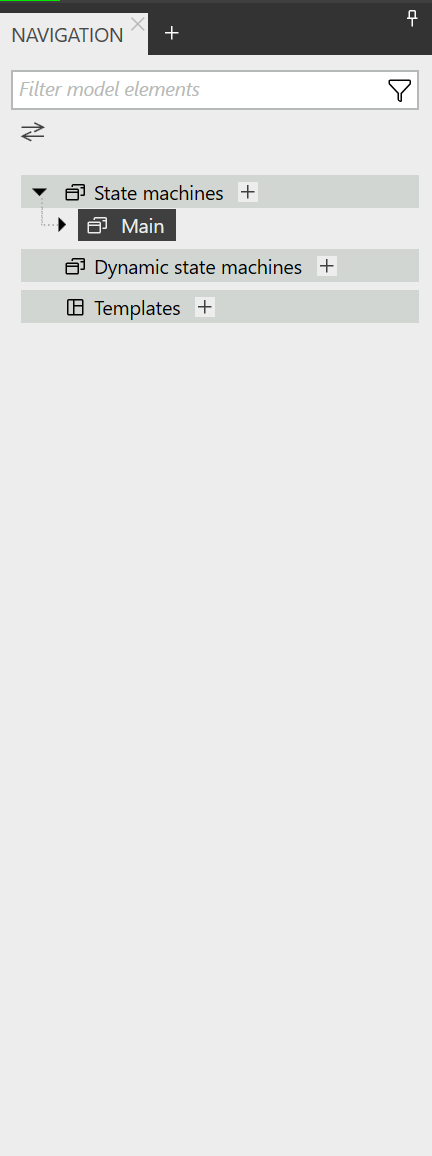
\includegraphics[scale=0.5]{figures/Navigation.png}
  \captionof{figure}{Usability - Schwäche Navigation}
  \label{fig:Navigation}
\end{center}


\paragraph{Template Properties}
Rechtsklick bei Widget Properties notwendig um Verlinkung zum Template Interface zu erstellen. Einfacher klick auf Kreis vorne?

\begin{center}
  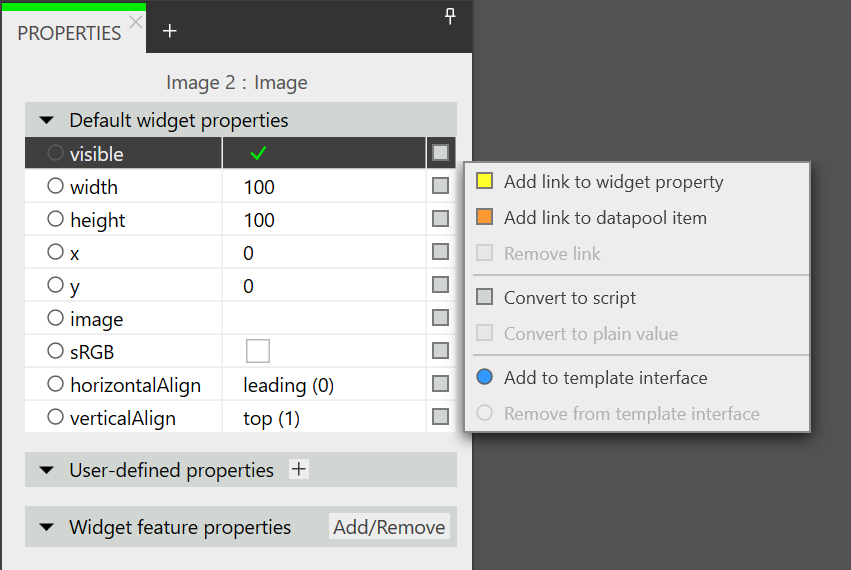
\includegraphics[scale=0.5]{figures/TemplateProperties.png}
  \captionof{figure}{Usability - Schwäche Template Properties}
  \label{fig:TemplateProperties}
\end{center}


\paragraph{Widget Feature Properties}
Häufiges Ausklappen der obermenüs bei der Suche nach bereits bekannten Features. Suche einbauen?

\begin{center}
  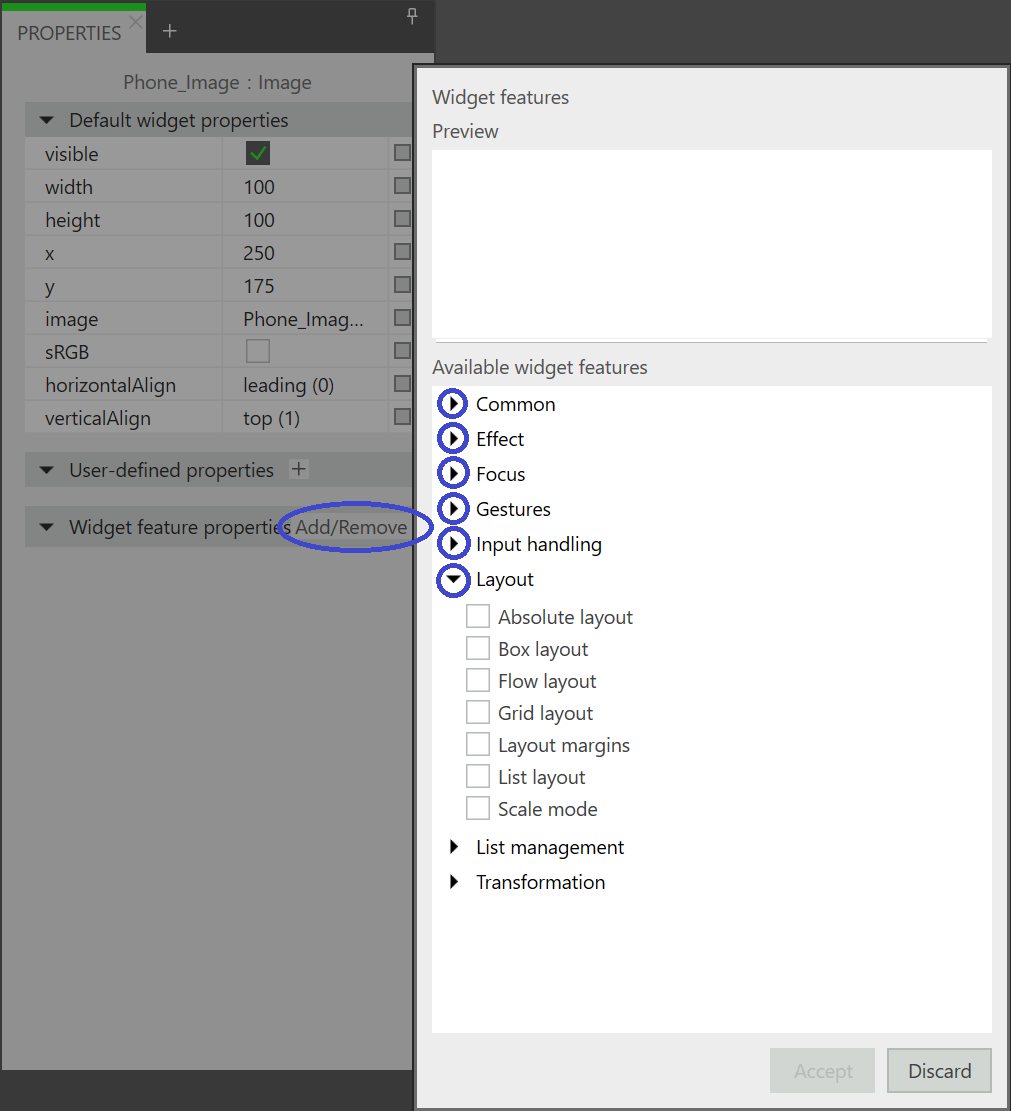
\includegraphics[scale=0.5]{figures/WidgetFeatureProperty.png}
  \captionof{figure}{Usability - Schwäche Widget Feature Properties}
  \label{fig:WidgetFeatureProperty}
\end{center}


\paragraph{Mehrfachselektion}
Bei Mehrfachselektion keine Anpassung der Properties mehr möglich. Im WidgetTree nicht sichbar was ausgewählt ist, hier ist eine mehrfache Markierung auch nicht möglich.

\begin{center}
  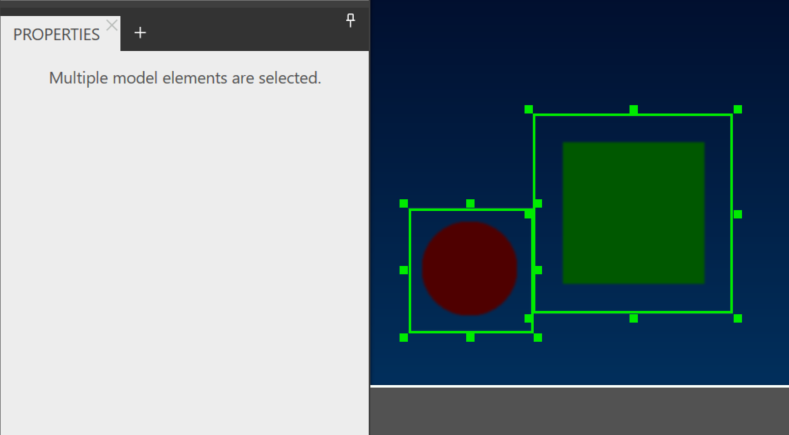
\includegraphics[scale=0.8]{figures/Mehrfachselektion.png}
  \captionof{figure}{Usability - Schwäche Mehrfachselektion}
  \label{fig:Mehrfachselektion}
\end{center}


\paragraph{Default Widget Properties}
Springen zum nächsten Property mit Enter/Pfeiltasten möglich, jedoch keine Markierung zur direkten Bearbeitung.
Auch hier keine Mehrfachselektion möglich, praktisch bei z.B quadratischen Bildern.
\begin{center}
  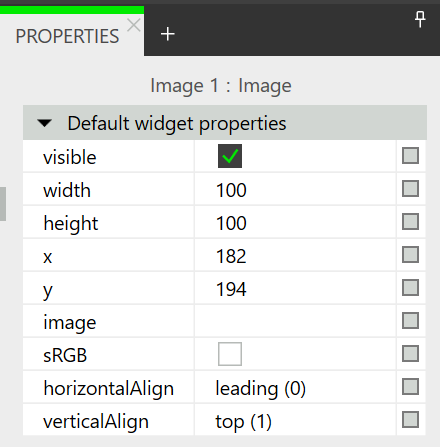
\includegraphics[scale=0.8]{figures/DefaultProperties.png}
  \captionof{figure}{Usability - Schwächen bei den Default Widget Properties}
  \label{fig:DefaultProperties}
\end{center}


\section{Verbesserungen}
\subsection{Auswahlkriterien}
\subsection{Gewinn für den Nutzer}
\subsection{Design der Verbesserungen}

\paragraph{Navigation}

\begin{center}
  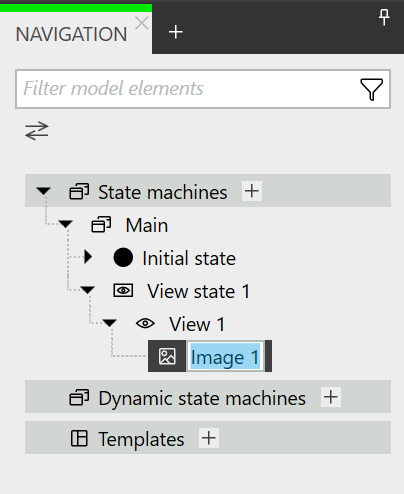
\includegraphics[scale=0.8]{figures/Navigation_Adaption.png}
  \captionof{figure}{Verbesserung Navigation}
  \label{fig:Navigation_Adaption}
\end{center}


\paragraph{Template Properties}

\begin{center}
  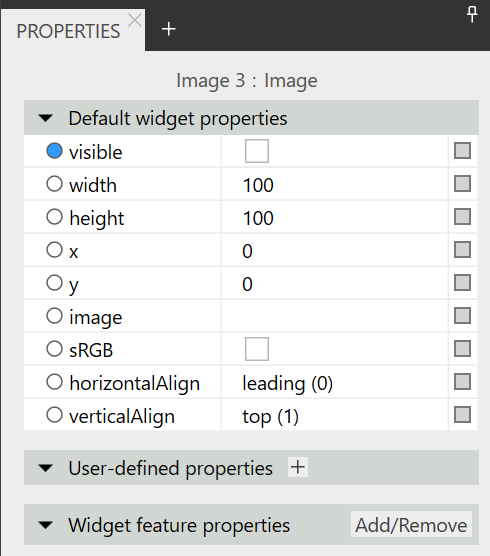
\includegraphics[scale=0.8]{figures/TemplateProperties_Adaption.png}
  \captionof{figure}{Verbesserung Template Properties}
  \label{fig:TemplateProperties_Adaption}
\end{center}


\paragraph{Widget Feature Properties}

\begin{center}
  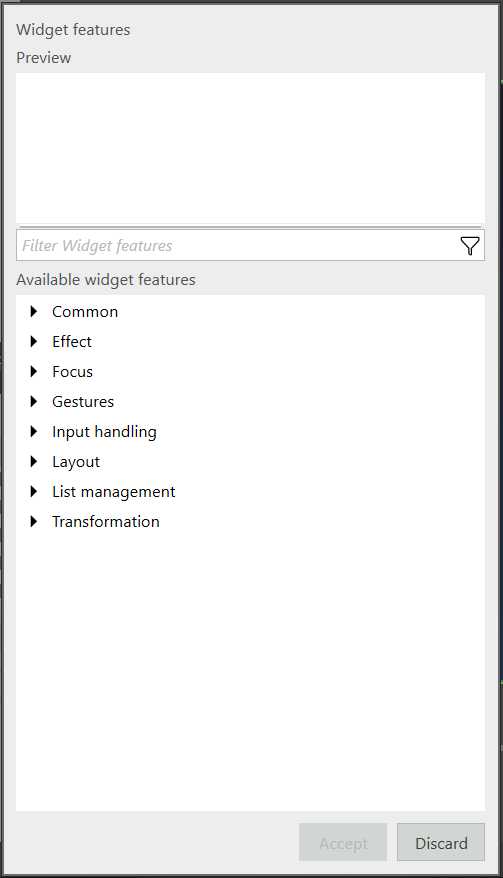
\includegraphics[scale=0.4]{figures/WidgetFeatureProperty_Adaption.png}
  \captionof{figure}{Verbesserung Feature Property Properties}
  \label{fig:FeatureProperty_Adaption}
\end{center}


\paragraph{Mehrfachselektion}

\begin{center}
  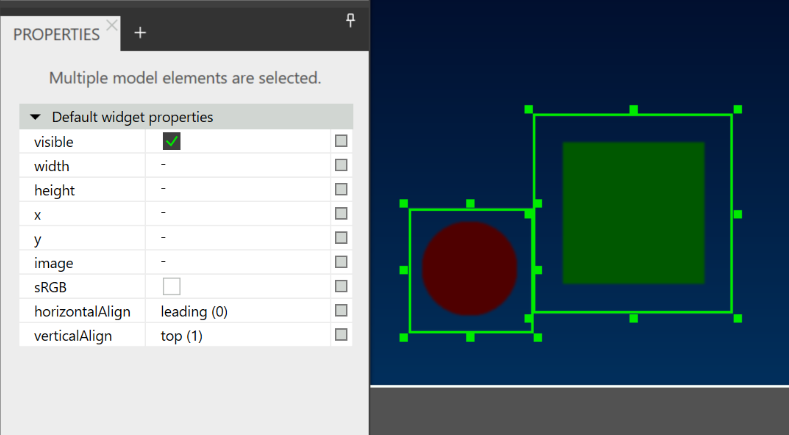
\includegraphics[scale=0.4]{figures/Mehrfachselektion_Adaption.png}
  \captionof{figure}{Verbesserung Mehrfachselektion}
  \label{fig:Mehrfachselektion_Adaption}
\end{center}


\paragraph{Default Widget Properties}

\begin{center}
  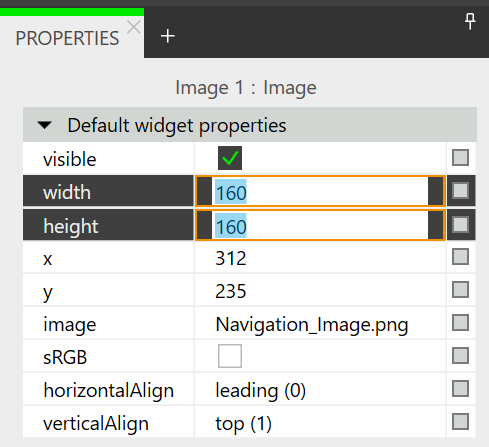
\includegraphics[scale=0.4]{figures/DefaultProperties_Adaption.png}
  \captionof{figure}{Verbesserung Default Widget Properties}
  \label{fig:DefaultProperties_Adaption}
\end{center}
